\documentclass{article}
    \usepackage{amsmath}
    \usepackage{amssymb}
    \usepackage{enumerate}
    \usepackage{graphicx}

    \usepackage{listings}
    \usepackage[usenames,dvipsnames]{xcolor}
    \usepackage{fontspec}
    \setmonofont{Courier New}
    \definecolor{mygreen}{rgb}{0,0.6,0}
    \definecolor{mygray}{rgb}{0.5,0.5,0.5}
    \definecolor{mymauve}{rgb}{0.58,0,0.82}
        \lstset{
            numbers = left, 
            basicstyle = \footnotesize\ttfamily,
            columns = fixed,
            breaklines = true, % automatic line breaking only at whitespace
            tabsize = 4,
            commentstyle = \color{mygreen},
            keywordstyle = \color{blue},
            stringstyle = \color{mymauve}\ttfamily,
            frame = lrbt,
            rulesepcolor = \color{red!20!green!20!blue!20},
            numbersep = -1em,
        }
    \usepackage{tikz}
        \usetikzlibrary{arrows}
        \usetikzlibrary{decorations.shapes}

    \newcommand{\sinc}{\text{sinc}}
    \renewcommand{\Re}{\text{Re}\hspace*{.2em}}
    \newcommand{\Res}{\Re s}

\begin{document}
\section*{EE 120 SIGNALS AND SYSTEMS, Fall 2019}
    \subsection*{Homework \#1}
        \begin{enumerate}
            \item Omitted.
            
            \item 
            \begin{enumerate}[(a)]
                \item stable, causal, FIR;
                \item unstable, causal, IIR;
                \item stable, non-causal, IIR;
                \item stable, causal, IIR.
            \end{enumerate}

            \item 
            \begin{enumerate}[(a)]
                \item Omitted.
                \item Omitted.
                \item Omitted.
                \item[(d)] When $x[n]$ is the unit impulse, the response is \[
                    h[n] = 1 + \sum_{k = 0}^{n} \delta[k],\ n > 0,
                \]
                and when the unit impulse is scaled by $\alpha$, the response is \[
                    \hat{h} [n] = 1 + \alpha\sum_{k = 0}^{n} \delta[k] \neq \alpha h[n].
                \]
                \item Linear and time-invariant.
            \end{enumerate}
            
            \item 
            \begin{enumerate}[(a)]
                \item \[
                    h[n] = \frac{1}{4}(\delta[n - 1] + 2\delta[n] + \delta[n + 1])
                \]
                \item \[
                    H(e^{j\omega}) = \sum\limits_{k=-\infty}^{\infty} h[k] e^{-jk\omega} = \frac{1 + \cos\omega}{2} = \cos^2 \frac{\omega}{2}
                \]
                \item Low-pass filter.
            \end{enumerate}	
            
            \item 
            \begin{enumerate}[(a)]
                \item \[
                    H(j\omega) = \frac{1}{1 + RC(j\omega)}
                \]
                \item \[
                    \left\vert H(j\omega) \right\vert = \frac{1}{\sqrt{1 + (RC\omega)^2}} 
                \]
                (The plot is omitted.)
            \end{enumerate}	
        \end{enumerate}
        \newpage
    
    \subsection*{Homework \#2}
        \begin{enumerate}
            \item \[
                \hat{a}_k = \frac{1}{jk\pi}[1 - (-1)^{k}] = 
                \begin{cases}
                    0,\ & k : \text{even} \\
                    \frac{2}{jk\pi},\ & k : \text{odd}.
                \end{cases}
            \]
            
            \item
            \begin{enumerate}[(a)]
                \item Omitted.
                \item Omitted.
                \item Omitted.
                \item Property (b) and (c). 
            \end{enumerate}	
            
            \item 
            \begin{enumerate}[(a)]
                \item The matrix elements are $w_{mn} = e^{j(m - 1) \frac{2\pi}{N} (n - 1)}$, $m, n = 1, 2, \cdots , N$. Denote $w = e^{j 2\pi / N}$, so that \[
                    W = \begin{bmatrix}
                        1 & 1 & \cdots & 1 \\
                        1 & w & \cdots & w^{N - 1}  \\
                        \vdots & \vdots &  & \vdots  \\
                        1 & w^{N-1} & \cdots & w^{(N - 1)^2}  \\
                    \end{bmatrix}.
                \]
                \item $(x[0], x[1], x[2])^T = (1, 0, 0)^T$, $w = e^{j 2\pi / 3}$, \[
                    \begin{bmatrix}
                        1 \\ 0 \\ 0
                    \end{bmatrix}
                    = \begin{bmatrix}
                        1 & 1 & 1 \\
                        1 & w & w^2 \\
                        1 & w^2 & w^4 \\
                    \end{bmatrix}
                    \begin{bmatrix} 
                        a_0 \\ a_1 \\ a_2
                    \end{bmatrix}
                    \Rightarrow\ 
                    \begin{bmatrix} 
                        a_0 \\ a_1 \\ a_2
                    \end{bmatrix}
                    = \begin{bmatrix} 
                        \frac{w^3}{(w-1)^2(w+1)} \\ -\frac{w}{(1-w)^2} \\ \frac{1}{(w-1)^2(w+1)}
                    \end{bmatrix}
                    = \frac{1}{3}\begin{bmatrix} 
                        1 \\ 1 \\ 1
                    \end{bmatrix}.
                \]
                \item \[
                    W^{-1} = \frac{1}{N}\begin{bmatrix}
                        1 & 1 & \cdots & 1 \\
                        1 & w^{-1} & \cdots & w^{-(N - 1)}  \\
                        \vdots & \vdots &  & \vdots  \\
                        1 & w^{-(N-1)} & \cdots & w^{-(N - 1)^2}  \\
                    \end{bmatrix}.
                \]
                \item Omitted.
            \end{enumerate}	
            
            \item Omitted.
            
            \item \[
                y(t) = s(t)\cos\varphi.
            \]
            when $\varphi = 90^\circ$, \[
                y(t) \equiv 0.
            \]
        \end{enumerate}
        \newpage
    
    \subsection*{Homework \#3}
        \begin{enumerate}
            \item
            \begin{enumerate}[(a)]
                \item $h_k = h^{(k)}(t)$.
                \item \[
                    H_1(\omega) = j\omega e^{-\omega^2 / 2},\ 
                    \left\vert H_1(\omega) \right\vert = \left\vert \omega \right\vert  e^{-\omega^2 / 2}.
                \]
                The plot of $\left\vert H_1(\omega) \right\vert $ is omitted.
                \item \[
                    H_\text{diff} (\omega) = j\omega,\ 
                    \left\vert H_\text{diff} (\omega) \right\vert = \left\vert \omega \right\vert. 
                \]
            \end{enumerate}	
            
            \item 
            \begin{enumerate}[(a)]
                \item Omitted.
                \item \[
                    H(e^{j\omega}) = -\frac{[2a - (1 + a^2) \cos\omega] - j(1 - a^2)\sin\omega}{1 - 2a\cos\omega + a^2},
                \]
                \[
                    \angle H(e^{j\omega}) = \pi + \arcsin[(1-a^2) \sin \omega].
                \]
                \item \[
                    y[n] = \cos\left( \frac{\pi}{6}n - \varphi\right) + \cos(n\pi - \pi),\ 
                    \varphi = \pi - \arcsin \frac{1}{3}.
                \]
                \item \[
                    y[n] - ay[n-1] = -ax[n] + x[n - 1].
                \]
            \end{enumerate}
            
            \item 
            \begin{enumerate}[(a)]
                \item $N = 103$.
                \item \ 
                \vspace{-1em}
                \begin{figure}[htbp]
                    \centering
                    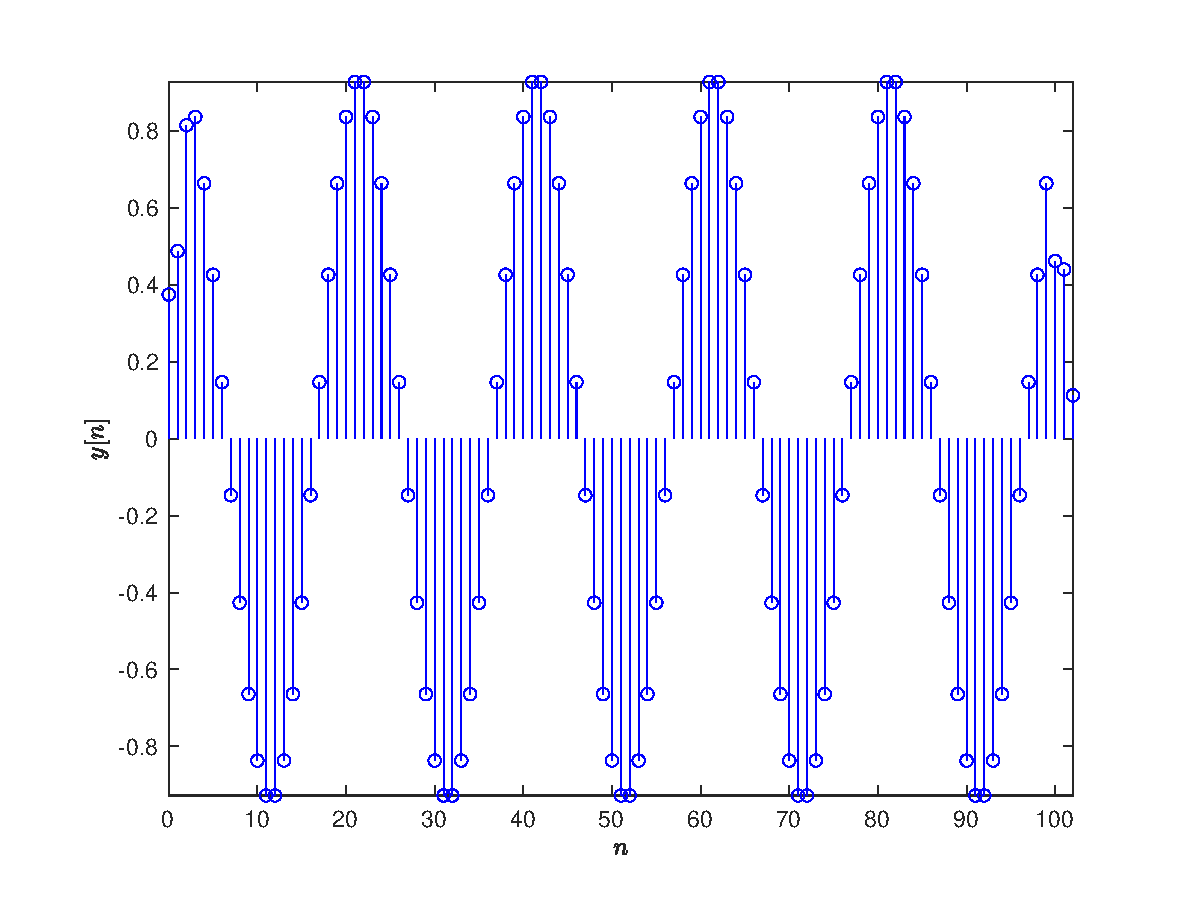
\includegraphics[width = .6\textwidth]{fig/fft}
                \end{figure}
            \end{enumerate}	
            % \vspace{-1em}
            \begin{lstlisting}[language = matlab]
    % matlab script
    x = zeros(103, 1);
    h = zeros(103, 1);
    xRange = (0 : 99)';
    x(1 : 100) = cos(0.1 * pi * xRange) + 0.5 * cos(pi * xRange);
    h(1 : 4) = 1 / 4;
    Y = fft(x) .* fft(h);
    y = ifft(Y);
    seriesPlot(y, 'b');
    xlabel('$n$', Interpreter='latex');
    ylabel('$y[n]$', Interpreter='latex');
    axis([0, 102, -Inf, Inf]);
            \end{lstlisting}
            % \vspace{.5em}
            \begin{lstlisting}[language = matlab]
    % matlab function
    function seriesPlot(x, color)
        n = length(x);
        range = 0 : n - 1;
        plot(range, x, strcat(color, 'o'));
        
        for i = 1 : n
            hold on;
            plot([range(i), range(i)], [0, x(i)], strcat(color, '-'));
        end
    end
            \end{lstlisting}

            \item 
            \begin{enumerate}[(a)]
                \item $h[n_1, n_2] = $ \[
                    \frac{
                        \delta[n_1, n_2] + 
                        \delta[n_1 - 1, n_2] + 
                        \delta[n_1 + 1, n_2] + 
                        \delta[n_1, n_2 - 1] + 
                        \delta[n_1, n_2 + 1]
                    }{5}.
                \]
                \item \[
                    H(e^{j\omega_1}, e^{j\omega_2}) = \frac{1}{5} (1 + 2\cos\omega_1 + 2\cos\omega_2).
                \]
                \vspace{-1em}
                \begin{figure}[htbp]
                    \centering
                    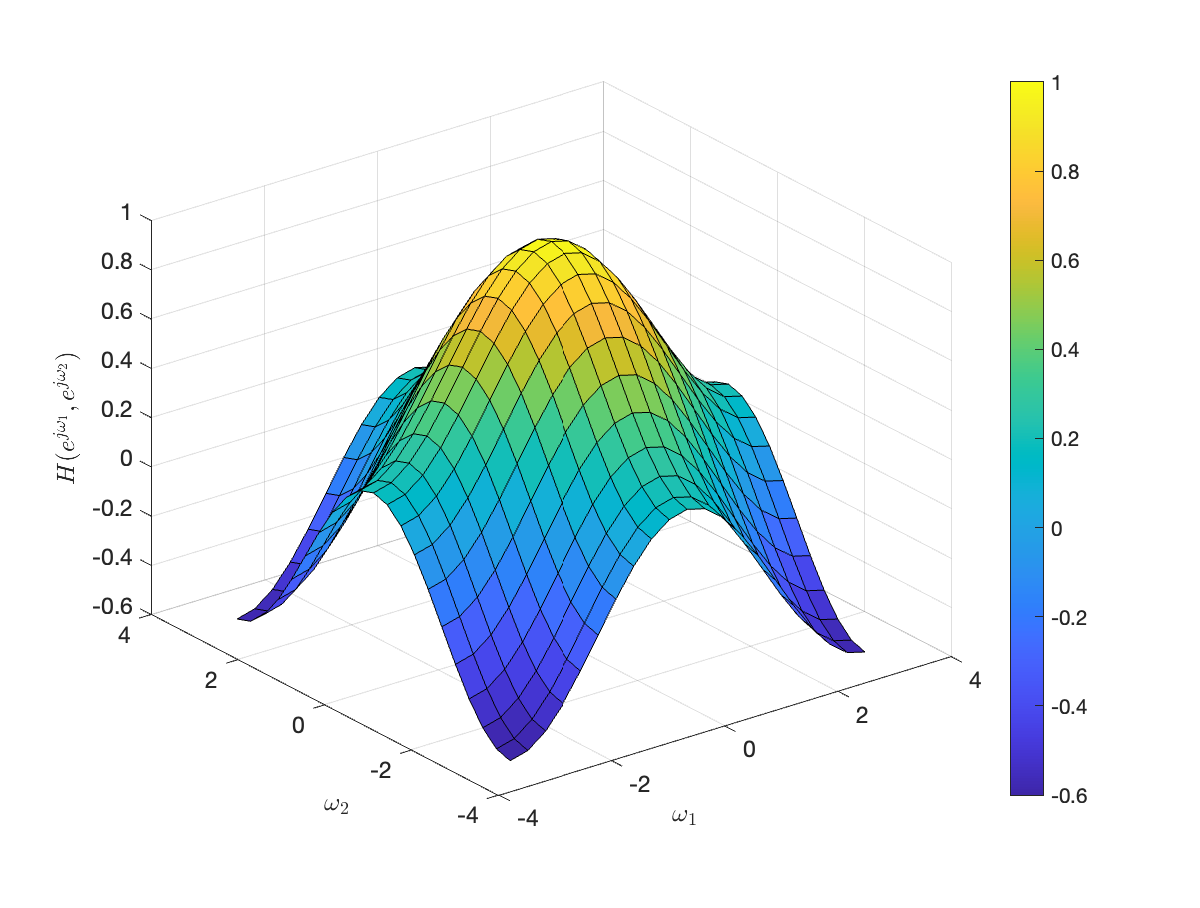
\includegraphics[width = .6\textwidth]{fig/dft}
                \end{figure}
            \end{enumerate}	
            \vspace{-1em}
            \begin{lstlisting}[language = matlab]
    % matlab code
    [omega1, omega2] = meshgrid(linspace(-pi, pi, 21));
    H = (1 + 2*cos(omega1) + 2*cos(omega2)) / 5;
    surf(omega1, omega2, H);
    xlabel('$\omega_1$', Interpreter='latex');
    ylabel('$\omega_2$', Interpreter='latex');
    zlabel('$H(e^{j\omega_1}, e^{j\omega_2})$', Interpreter='latex');
            \end{lstlisting}
            
            \item Omitted.
        \end{enumerate}
        \newpage

    \subsection*{Homework \#4}
        \begin{enumerate}
            \item The angular velocity is \[
                \omega = 12(3 + 4k) \pi\ \text{s}^{-1},\ k = 0, 1, \cdots.
            \]
            
            \item 
            \begin{enumerate}[(a)]
                \item 19 kHz.
                \item The plots of $X_p(\omega)$ and the reconstruction filter's frequency response $H_r(\omega)$ are as below.
                \vspace{-1em}
                \begin{figure}[htbp]
                    \tiny
                    \centering
                    \hspace*{6em}
                    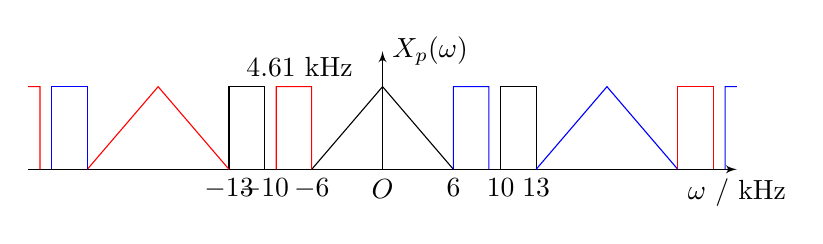
\begin{tikzpicture} [scale = 1.5]
    \draw[-latex'] (-3, 0) -- (3, 0) node[below = 0] {$\omega$ / kHz};
    \draw[-latex'] (0, 0) node[below = 0] {$O$} 
        -- (0, 1) node[right = 0] {$X_p(\omega)$};

    \draw (0, 0.7) node[above = 0] {4.61 kHz\hspace*{6em}} 
        -- (0.6, 0) node[below = 0] {6};
    \draw (0, 0.7) -- (-0.6, 0) node[below = 0] {$-6$};
    \draw (-1.0, 0) node[below = 0] {$-10$} -- (-1.0, 0.7) -- (-1.3, 0.7)
        -- (-1.3, 0) node[below = 0] {$-13$};
    \draw (1.0, 0) node[below = 0] {$10$} -- (1.0, 0.7) -- (1.3, 0.7)
        -- (1.3, 0) node[below = 0] {$13$};

    \draw[red] (-0.6, 0) -- (-0.6, 0.7) -- (-0.9, 0.7) -- (-0.9, 0)
        (-1.3, 0) -- (-1.9, 0.7) -- (-2.5, 0)
        (-2.9, 0) -- (-2.9, 0.7) -- (-3.0, 0.7);
    \draw[blue] (0.6, 0) -- (0.6, 0.7) -- (0.9, 0.7) -- (0.9, 0)
        (1.3, 0) -- (1.9, 0.7) -- (2.5, 0)
        (2.9, 0) -- (2.9, 0.7) -- (3.0, 0.7);    

    % 补充
    \draw[blue] (-2.5, 0) -- (-2.5, 0.7) -- (-2.8, 0.7) -- (-2.8, 0);
    \draw[red] (2.5, 0) -- (2.5, 0.7) -- (2.8, 0.7) -- (2.8, 0);
\end{tikzpicture}
                    \vspace{-4em}
                    \hspace*{6em}
                    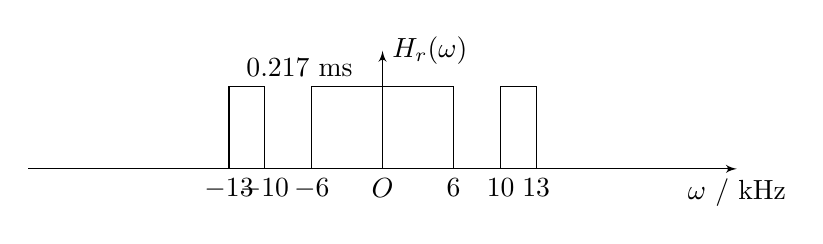
\begin{tikzpicture} [scale = 1.5]
    \draw[-latex'] (-3, 0) -- (3, 0) node[below = 0] {$\omega$ / kHz};
    \draw[-latex'] (0, 0) node[below = 0] {$O$} 
        -- (0, 1) node[right = 0] {$H_r(\omega)$};
    
    \draw (-0.6, 0) node[below = 0] {$-6$} -- (-0.6, 0.7) 
        -- (0, 0.7) node[above = 0] {0.217 ms\hspace*{6em}}
        -- (0.6, 0.7) -- (0.6, 0) node[below = 0] {6};
    \draw (-1.0, 0) node[below = 0] {$-10$} -- (-1.0, 0.7) -- (-1.3, 0.7)
        -- (-1.3, 0) node[below = 0] {$-13$};
    \draw (1.0, 0) node[below = 0] {$10$} -- (1.0, 0.7) -- (1.3, 0.7)
        -- (1.3, 0) node[below = 0] {$13$};
\end{tikzpicture}
                \end{figure}
            \end{enumerate}	

            \item 
            \begin{enumerate}[(a)]
                \item Omitted.
                \item $x_r(t) = 1$.
                \item $\hat{x}_r(t) = -1 \neq x_r(t - \frac{1}{2})$.
            \end{enumerate}	
            
            \item 
            \begin{enumerate}[(a)]
                \item \[
                    h_d[n] = \begin{cases}
                        \frac{1}{nT} ,\ & n \neq 0, \\
                        \frac{\pi j}{T},\ & n = 0.
                    \end{cases}
                \]
                \item ? \[
                    \hat{H}_d(e^{j \Omega}) = \frac{\alpha j}{T} (\pi - 2\sin \Omega),\ \alpha = -\frac{1}{2}.
                \]
                \item ? \[
                    y_d[n] = -\frac{1}{2T}(j\pi x[n] - x[n + 1] + x[n - 1]).
                \]
            \end{enumerate}	
            
            \item 
            \begin{enumerate}[(a)]
                \item \[
                    X_p(e^{j\omega_1}, e^{j\omega_2}) = \frac{1}{N_1N_2} \sum\limits_{k_1=0}^{N_1 - 1} \sum\limits_{k_2=0}^{N_2 - 1} X(e^{j(\omega_1 - k_1 \frac{2\pi}{N_1})},e^{j(\omega_2 - k_2 \frac{2\pi}{N_2})}). 
                \]
                \item $\frac{2\pi}{N_1} > 2 \omega_{M1}$ and $\frac{2\pi}{N_2} > 2\omega_{M 2}$, where $\omega_{M 1}, \omega_{M 2}$ satisfy \[
                    X(e^{j\omega_1}, e^{j\omega_2}) = 0,\ 
                    \omega_{M 1} < \left\vert \omega_1 \right\vert \le \pi,\ 
                    \omega_{M 2} < \left\vert \omega_2 \right\vert \le \pi.
                \]
                \item \[
                    h_r[n_1, n_2] = \sinc\left( \frac{n_1}{N_1}\right) \sinc\left( \frac{n_1}{N_2}\right).
                \]
            \end{enumerate}	
        \end{enumerate}
        \newpage

    \subsection*{Homework \#5}
        \begin{enumerate}
            \item 
            \begin{enumerate}[(a)]
                \item \[
                    X(s) = \frac{s+1}{s^2 +2s+5},\ \Res > -1.
                \]
                \item \[
                    X(s) = -\frac{1}{s^2 +1},\ \Res <0.
                \]
                \item \[
                    X(s) = \frac{s^2 -1}{s^2 +1},\ \Res > 0.
                \]
                \item \[
                    X(s) = e^{-s},\ s \in \mathbb{C}.
                \]
            \end{enumerate}	
            
            \item 
            \begin{enumerate}[(a)]
                \item \[
                    x(t) = e^{-2t} \cos t u(t).  
                \]
                \item \[
                    x(t) = \cos(t - 1) u(t - 1).  
                \]
                \item \[
                    x(t) = \frac{1}{2}t\sin t u(t).  
                \]
                \item \[
                    x(t) = (-e^{-3t} + 2 e^{-4 t})u(t).  
                \]
            \end{enumerate}
            
            \item 
            \begin{enumerate}[(a)]
                \item Omitted.
                \item (c) If the input $x(t) = \cos\omega_nt u(t)$, which is bounded, then \[
                    Y(s) = H(s)X(s) = \frac{\omega_n^2 }{s^2 +\omega_n^2 }\cdot \frac{s}{s^2 +\omega_n^2} = \frac{\omega_n^2 s}{(s^2 +\omega_n^2)^2}.
                \]
                Use the results in 2(c), and we can get an unbounded output: \[
                    y(t) = \frac{1}{2}\omega_nt\sin\omega_nt u(t).
                \]
                \item[(d)] Omitted.
            \end{enumerate}
            
            % \item See Figure \ref{fig:bode}.
            \item See Figure 1.

            \item 
            \begin{enumerate}[(a)]
                \item \[
                    H(s) = \frac{b_0 + b_1s}{a_0 + a_1 s + s^2}.
                \]
                \item \[
                    H(s) = \frac{b_0 + b_1s}{a_0 + a_1 s + s^2}.
                \]
            \end{enumerate}	
            
            \item Denote $y(t) \fallingdotseq Y(p)$, then \[
                \dot{y}(t) \fallingdotseq pY(p) - \frac{5}{2},\ 
                \ddot{y}(t) \fallingdotseq p^2 Y(p) - \frac{5}{2} p + \frac{9}{2},\ 
                x(t) \fallingdotseq \frac{1}{p+3},
            \]
            and \[
                Y(p) = \frac{\frac{5}{2}p^2 + \frac{21}{2} p + 10}{(p+1)(p+2)(p+3)}
                = \frac{1}{p+1} + \frac{1}{p+2} + \frac{1 / 2}{p+3}.
            \]
            \[
                \Rightarrow\ y(t) = \left( e^{-t} + e^{-2t} + \frac{1}{2}e^{-3t}\right) u(t).
            \]
            
        \end{enumerate}
        
        \vspace{2em}
        \begin{figure}[htbp]
            \centering
            \begin{minipage}{.49\textwidth}
                \centering
                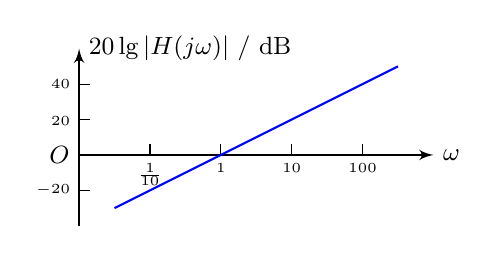
\begin{tikzpicture}[scale = .45]
    \small
    %% axis
    \draw[-latex', thick] (0, -2) -- (0, 3) node[right = 0] {$20\lg |H(j\omega)|$ / dB};
    \draw[-latex', thick] (0, 0) node[left = 0] {$O$} 
        -- (10, 0) node[right = 0] {$\omega$};

    %% scale
    \draw (2, 0) node[below = 0] {\tiny $\frac{1}{10}$} -- +(0, 0.3);
    \draw (4, 0) node[below = 0] {\tiny $1$} -- +(0, 0.3);
    \draw (6, 0) node[below = 0] {\tiny $10$} -- +(0, 0.3);
    \draw (8, 0) node[below = 0] {\tiny $100$} -- +(0, 0.3);

    \draw (0, 1) node[left = 0] {\tiny $\phantom{^\circ}20$} -- +(0.3, 0);
    \draw (0, 2) node[left = 0] {\tiny $40$} -- +(0.3, 0);
    \draw (0, -1) node[left = 0] {\tiny $-20$} -- +(0.3, 0);

    %% curve
    \draw[blue, thick] (4, 0) -- +(5, 2.5) (4, 0) -- +(-3, -1.5);
\end{tikzpicture} 

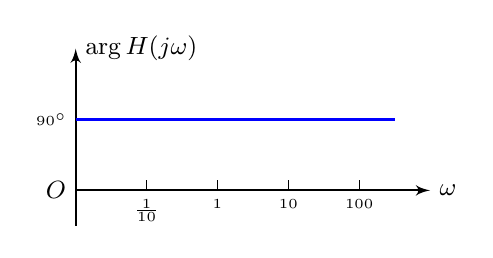
\begin{tikzpicture}[scale = .45]
    \small
    %% axis
    \draw[-latex', thick] (0, -1) -- (0, 4) node[right = 0] {$\arg H(j\omega)$};
    \draw[-latex', thick] (0, 0) node[left = 0] {$O$} 
        -- (10, 0) node[right = 0] {$\omega$};

    %% scale
    \draw (2, 0) node[below = 0] {\tiny $\frac{1}{10}$} -- +(0, 0.3);
    \draw (4, 0) node[below = 0] {\tiny $1$} -- +(0, 0.3);
    \draw (6, 0) node[below = 0] {\tiny $10$} -- +(0, 0.3);
    \draw (8, 0) node[below = 0] {\tiny $100$} -- +(0, 0.3);
    % \draw (0, 1.5) node[left = 0] {\tiny $45^\circ$} -- +(0.3, 0);
    \draw (0, 2.0) node[left = 0] {\tiny $90^\circ$} -- +(0.3, 0);

    %% curve
    \draw[blue, thick] (0, 2) -- (9, 2);
\end{tikzpicture}



                \vspace{-2em}
                (a)
            \end{minipage}
            \begin{minipage}{.49\textwidth}
                \centering
                \include{tikzs/BodePlot2.tex}
                \vspace{-2em}
                (b)
            \end{minipage}
            \begin{minipage}{.49\textwidth}
                \centering
                \include{tikzs/BodePlot3.tex}
                \vspace{-2em}
                (c)
            \end{minipage}
            \begin{minipage}{.49\textwidth}
                \centering
                \vspace{.5em}
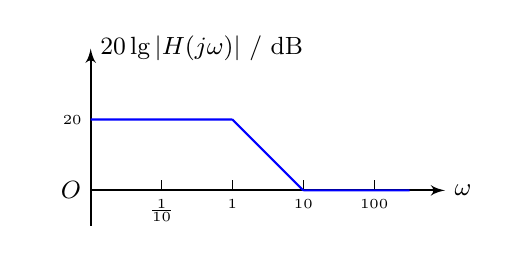
\begin{tikzpicture}[scale = .45]
    \small
    %% axis
    \draw[-latex', thick] (0, -1) -- (0, 4) node[right = 0] {$20\lg |H(j\omega)|$ / dB};
    \draw[-latex', thick] (0, 0) node[left = 0] {$O$} 
        -- (10, 0) node[right = 0] {$\omega$};

    %% scale
    \draw (2, 0) node[below = 0] {\tiny $\frac{1}{10}$} -- +(0, 0.3);
    \draw (4, 0) node[below = 0] {\tiny $1$} -- +(0, 0.3);
    \draw (6, 0) node[below = 0] {\tiny $10$} -- +(0, 0.3);
    \draw (8, 0) node[below = 0] {\tiny $100$} -- +(0, 0.3);
    \draw (0, 2) node[left = 0] {\tiny $\phantom{-^\circ}20$} -- +(0.3, 0);

    %% curve
    \draw[blue, thick] (0, 2) -- (4, 2) (4, 2) -- (6, 0) (6, 0) -- (9, 0);
\end{tikzpicture} 

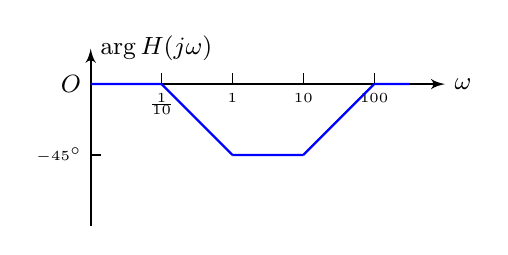
\begin{tikzpicture}[scale = .45]
    \small
    %% axis
    \draw[-latex', thick] (0, -4) -- (0, 1) node[right = 0] {$\arg H(j\omega)$};
    \draw[-latex', thick] (0, 0) node[left = 0] {$O$} 
        -- (10, 0) node[right = 0] {$\omega$};

    %% scale
    \draw (2, 0) node[below = 0] {\tiny $\frac{1}{10}$} -- +(0, 0.3);
    \draw (4, 0) node[below = 0] {\tiny $1$} -- +(0, 0.3);
    \draw (6, 0) node[below = 0] {\tiny $10$} -- +(0, 0.3);
    \draw (8, 0) node[below = 0] {\tiny $100$} -- +(0, 0.3);
    \draw (0, -2) node[left = 0] {\tiny $-45^\circ$} -- +(0.3, 0);

    %% curve
    \draw[blue, thick] (0, 0) -- (2, 0) (2, 0) -- (4, -2) (4, -2) -- (6, -2)
        (6, -2) -- (8, 0) (8, 0) -- (9, 0);
\end{tikzpicture}

                \vspace{-2em}
                (d)
            \end{minipage}
            %
            % \addtocounter{figure}{+3}
            % \label{fig:bode}
            \caption{The Bode plots of problem 4}
        \end{figure}
        \newpage
        
    \subsection*{Homework \#6}
        \begin{enumerate}
            \item \[
                x[n] = \left[ -\frac{5}{3}\left( -\frac{1}{2}\right)^{n} + \frac{8}{3} (-2)^{n} \right] u[n].
            \]
            
            \item 
            \begin{enumerate}[(a)]
                \item \[
                    H(z) = \frac{1}{1-\frac{3}{2}z^{-1} + \frac{1}{2}z^{-2}},\ 
                    |z| > 1.
                \]
                \item Unstable.
                \item \[
                    y[n] = \left[ \left( \frac{1}{2}\right)^{n} + 2n\right] u[n].
                \]
            \end{enumerate}	
            
            \item 
            \begin{enumerate}[(a)]
                \item Stable. (
                    \tikz\draw[decorate, decoration = {crosses, shape size = 5pt}, thick, blue] (0, 0);\hspace*{.2em}
                    for poles and \
                    \tikz\draw[thick, blue] (0, 0) circle(2pt);\hspace*{.2em}
                    for zeros in the figure below.%
                )
                \vspace{-1em}
                \begin{figure}[htbp]
                    \centering
                    \begin{minipage}{.35\textwidth}
                        \centering
                        \vspace{3em}
                        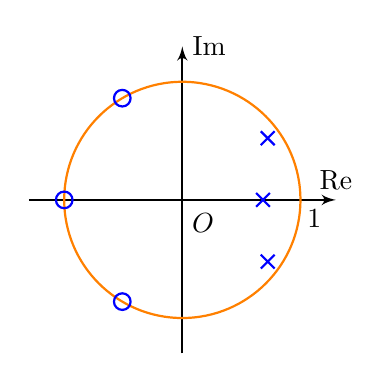
\begin{tikzpicture}[scale = 1.5]
    \draw[thick, -latex'] (-1.3, 0) -- (1.3, 0) node[above = 0] {Re};
    \draw[thick, -latex'] (0, -1.3) -- (0, 1.3) node[right = 0] {Im};
    \draw[thick, orange] (0, 0) circle(1);
    
    \path (0, -0.2) node[right = 0] {$O$};
    \path (1, 0) node[below = 0] {\quad $1$};

    %% poles
    \draw[decorate, decoration = {crosses, shape size = 5pt}, thick, blue]
        (0.683, 0);
    \draw[decorate, decoration = {crosses, shape size = 5pt}, thick, blue]
        (0.723, 0.5224);
    \draw[decorate, decoration = {crosses, shape size = 5pt}, thick, blue]
        (0.723, -0.5224);
        
    %% zeros
    \draw[thick, blue] (-1, 0) circle(2pt);
    \draw[thick, blue] (-0.5083, 0.8612) circle(2pt);
    \draw[thick, blue] (-0.5083, -0.8612) circle(2pt);
\end{tikzpicture}
                        \vspace{-2em}
                        (a)
                    \end{minipage}
                    \begin{minipage}{.64\textwidth}
                        \centering
                        \includegraphics[width = .99\textwidth]{fig/hz.eps}
                        % \vspace{-2em}
                        (b)
                    \end{minipage}
                \end{figure}
            \end{enumerate}	
            
            \item
            \begin{enumerate}[(a)]
                \item $\omega_0 = \arccos \beta$.
                \item Omitted.
            \end{enumerate}

            \item 
            \begin{enumerate}[(a)]
                \item Omitted.
                \item $H_\text{bp} (e^{j 0}) = H_\text{bp}(e^{j\pi}) = 0$, $H_\text{bp}(e^{j\omega_0}) = 1$.
            \end{enumerate}	
            
            \item \[
                H(z) = \frac{(b_1-a_1b_0)z^{-1} + (b_2-a_2b_0)z^{-2}}{1 + a_1z^{-1} + a_2z^{-2}} + b_0.
            \]
            
            \item \[
                Y(z) = \frac{2 - \frac{3}{2}z^{-1}}{(1-z^{-1})(1-\frac{1}{2}z^{-1})}
                = \frac{1}{1-z^{-1}} + \frac{1}{1-\frac{1}{2}z^{-1}},
            \]
            \[
                y[n] = 1 + \left( \frac{1}{2}\right)^{n}.
            \]
        \end{enumerate}
        

\end{document}
